\documentclass[11pt,a4paper]{article}
%!TEX encoding = UTF-8 Unicode
%!TEX TS-program = pdflatex
%!TEX spellcheck = English
\usepackage{etex}
\usepackage[utf8]{inputenc}
\usepackage[TS1,T1]{fontenc}
\usepackage{textcomp}
\usepackage[a4paper,tmargin=3cm,bmargin=3cm,rmargin=2.2cm,lmargin=2.2cm]{geometry}
\usepackage{lmodern}
\usepackage{mathrsfs}
\usepackage{float}
\usepackage{enumerate}

\usepackage{amsfonts,amssymb,amsmath,mathtools,cite,slashed,cases}
\usepackage[amsthm,thmmarks,amsmath]{ntheorem}
% \usepackage{slashed}
%\usepackage{amsfonts,amssymb,amsmath,amsthm,cite,mathtools,cases}
\usepackage{graphicx}
\usepackage{hyperref}
\usepackage{xcolor}
\usepackage{listings} % to include code
\usepackage{etoolbox} 

\definecolor{mygreen}{rgb}{0,0.6,0}
\definecolor{mygray}{rgb}{0.47,0.47,0.33}
\definecolor{myorange}{rgb}{0.8,0.4,0}
\definecolor{mywhite}{rgb}{0.98,0.98,0.98}
\definecolor{myblue}{rgb}{0.01,0.61,0.98}

\newcommand*{\FormatDigit}[1]{\ttfamily\textcolor{mygreen}{#1}}
%% http://tex.stackexchange.com/questions/32174/listings-package-how-can-i-format-all-numbers
\lstdefinestyle{FormattedNumber}{%
    literate=*{0}{{\FormatDigit{0}}}{1}%
             {1}{{\FormatDigit{1}}}{1}%
             {2}{{\FormatDigit{2}}}{1}%
             {3}{{\FormatDigit{3}}}{1}%
             {4}{{\FormatDigit{4}}}{1}%
             {5}{{\FormatDigit{5}}}{1}%
             {6}{{\FormatDigit{6}}}{1}%
             {7}{{\FormatDigit{7}}}{1}%
             {8}{{\FormatDigit{8}}}{1}%
             {9}{{\FormatDigit{9}}}{1}%
             {.0}{{\FormatDigit{.0}}}{2}% Following is to ensure that only periods
             {.1}{{\FormatDigit{.1}}}{2}% followed by a digit are changed.
             {.2}{{\FormatDigit{.2}}}{2}%
             {.3}{{\FormatDigit{.3}}}{2}%
             {.4}{{\FormatDigit{.4}}}{2}%
             {.5}{{\FormatDigit{.5}}}{2}%
             {.6}{{\FormatDigit{.6}}}{2}%
             {.7}{{\FormatDigit{.7}}}{2}%
             {.8}{{\FormatDigit{.8}}}{2}%
             {.9}{{\FormatDigit{.9}}}{2}%
             %{,}{{\FormatDigit{,}}{1}% depends if you want the "," in color
             {\ }{{ }}{1}% handle the space
             ,%
}


\lstset{%
  backgroundcolor=\color{mywhite},   
  basicstyle=\footnotesize,       
  breakatwhitespace=false,         
  breaklines=true,                 
  captionpos=b,                   
  commentstyle=\color{red},    
  deletekeywords={...},           
  escapeinside={\%*}{*)},          
  extendedchars=true,              
  frame=shadowbox,                    
  keepspaces=true,                 
  keywordstyle=\color{myorange},       
  language=Octave,                
  morekeywords={*,...},            
  numbers=left,                    
  numbersep=5pt,                   
  numberstyle=\tiny\color{mygray}, 
  rulecolor=\color{black},         
%   rulesepcolor=\color{gray},
  showspaces=false,                
  showstringspaces=false,          
  showtabs=false,                  
  stepnumber=0,                    
  stringstyle=\color{myorange},    
  tabsize=2,                       
  title=\lstname,
  emphstyle=\bfseries\color{blue},%  style for emph={} 
}    

%% language specific settings:
\lstdefinestyle{Arduino}{%
    style=FormattedNumber,
    keywords={void},%                 define keywords
    morecomment=[l]{//},%             treat // as comments
    morecomment=[s]{/*}{*/},%         define /* ... */ comments
    emph={HIGH, OUTPUT, LOW},%        keywords to emphasize
}

\newtoggle{InString}{}% Keep track of if we are within a string
\togglefalse{InString}% Assume not initally in string

% 
%  \newcommand{\PAYE}{{\Large\color{orange}\checkmark}}
%  \newcommand{\RECU}{{\Large\color{green}\checkmark}}
% 


\usepackage{titlesec}
%\titleformat{\section}{\normalfont\scshape}{\thesection}{1em}{}
\titleformat{\section}[block]{\LARGE\bfseries\filcenter}{\thesection}{1em}{}
\titleformat{\subsection}[block]{\Large\bfseries\filcenter}{\thesubsection}{1em}{}
\titleformat{\subsubsection}[block]{\large\bfseries\filcenter}{\thesubsubsection}{1em}{}

%\newtheorem{remarque}{Remarque}
\newtheorem*{remarque*}{Remarque}



%%%%%%%%%%%%
% DOCUMENT %
%%%%%%%%%%%%

\title{Guide de fabrication ROV}

\begin{document}
  \maketitle
  \tableofcontents
%   \maketableofcontents
  
  \section{Description}
    \begin{figure}[H]
      \centering
      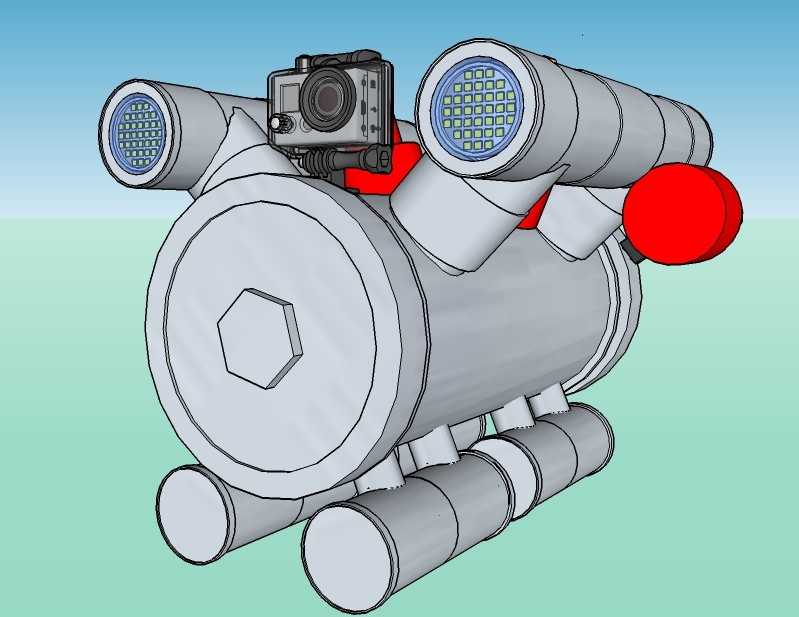
\includegraphics[scale=0.3]{ROVFinal.jpg}
      \caption{Aperçu global.}
    \end{figure}
    \begin{figure}[H]
      \centering
      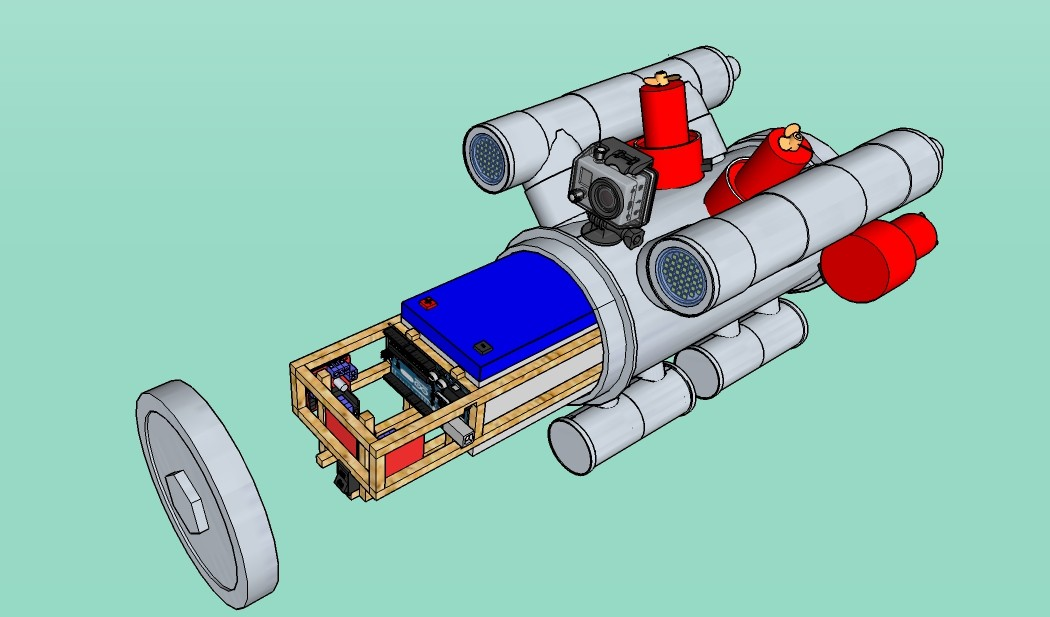
\includegraphics[scale=0.3]{ROVOuvert.jpg}
      \caption{ROV ouvert.}
    \end{figure}
    

  
  \section{Remarques diverses}
    \begin{itemize}
      \item Les pièces citées ci-dessous correspondent à ce modèle de ROV précis. Elles ont été modifiées au fur et à mesure de la conception. Bien que la majeure partie des plans aient été dessinés avant la fabrication, des détails pratiques subsistent toujours. En règle générale, faire les plans \underline{en détail} à l'avance réduit les mauvaises surprises.
    
      \item Lorsque vous choisissez ou fabriquez vos pièces, veillez à ce que toutes dimensions soient compatibles. Par exemple, la batterie que j'ai choisie rentre tout juste dans la coque (des rainures ont même dû être faites pour la glisser à l'intérieur).
      
      \item Les dimensions du ROV ne doivent être 
      \begin{itemize}
        \item \underline{ni trop grandes} : beaucoup de plomb à ajouter lors de l'étape de stabilisation pour compenser le gros volume, donc un ROV final très lourd
        \item \underline{ni trop petites} : un manque d'espace à l'intérieur du ROV réduit la marge de manoeuvre lors d'un problème pratique (oubli d'un composant, etc.). Prévoyez assez d'espace pour les fils.
      \end{itemize}
      
    
    \end{itemize}

  \section{Pièces}

  
    \subsection{Coque et support interne}
      \begin{itemize}
      \setlength\itemsep{-2mm}
       \item Pièces en PVC :
              \begin{center}
                \begin{tabular}{|c|c|c|c|}
                  \hline
                  \textbf{Quantité} & \textbf{Type} & \textbf{Longueur (mm)} & \textbf{Diamètre (mm)}\\
                  \hline
                  1 & Tube droit & 150 & 140\\
                  \hline
                  2 & Manchon & & 140\\
                  \hline
                  2 & Bouchon de visite & & 140\\
                  \hline
                  4 & Tube en T & & 50\\
                  \hline
                  4 & Bouchon de visite & & 50\\
                  \hline
                  2 & Manchon & & 50\\
                  \hline
                  8 & Tube droit & 40 & 50\\
                  \hline
                  8 & Bouchon visite & & 40\\
                  \hline
                  8 & Manchon & & 40\\
                  \hline
                  10 & Tube en T & & 40\\
                  \hline
                  1 & Tube droit & 50 & 32\\
                  \hline
                  8 & Tube droit & 20 & 32\\
                  \hline
                \end{tabular}
              \end{center}
        \item du plomb pour lester (plomb de 1/2 Kg pour la chasse sous-marine)
        \item 2 baguettes en bois de 2m, dimensions 50mm x 50mm
        \item 1 plaque de plexyglass épaisseur 3mm
      \end{itemize}

      
    \subsection{Électronique et connectique}
      \begin{itemize}
        \setlength\itemsep{-2mm}
        \item 1 carte compatible Arduino Mega2560 REV3 \cite{arduino}
        \item fils (mâle/mâle)
        \item 1 interrupteur
        \item 2 connecteurs molex 4 broches (1 femelle et 1 mâle)
        \item 2 joysticks analogiques (axes X/Y + boutton central) \cite{joystick}
        \item 2 câbles cat6 RJ45 : 1 rouleau de 50m et un autre de longueur quelconque
        \item 3 adaptateurs d'extension de câble cat6 RJ45 femelle/femelle
        \item 3 dual H-bridge %(30g Taille: 43 * 43 * 27mm)
        \item 2 spots blancs DEL 5W 12V DC (310-320 lumens) \cite{lampe}
        \item 1 batterie rechargeable 12V 12 A.h de dimensions 151mm x 98mm x 95mm
        \item 1 module de régulation de tension LM2596 DC 1.3--37V \cite{regulateurTension}%Converter Module LM2596 DC 4.0 ~ 40 à 1.3-37 V Tension Réglable régulateur
      \end{itemize}

    \subsection{Propulsion}
%      \KF{diamètres à check}
      \begin{itemize}
        \setlength\itemsep{-2mm}
        \item 4 pompes à cale 12V DC 1100GPH \cite{pompe}
        \item 4 hélices 43x26x9mm, diamètre de l'arbre 4mm \cite{helice}
        \item 4 drive dog 3.18mm \cite{driveDog}
        \item 4 sections tige filetée longueur 20mm diamètre 4mm %\cite{tigeFiletee}
        \item 4 adaptateurs d'axe diamètre 4mm \cite{adaptateurAxe}
        \item 4 colliers de serrage plastique
      \end{itemize}
      
    \subsection{Outils et consommables}
      \begin{itemize}
        \setlength\itemsep{-2mm}
        \item scies à bois et à métaux
        \item tournevis
        \item lime
        \item papier de verre
        \item dremel
        \item fer à souder
        \item étain
        \item pinces plates/coupantes
        \item 1 pot de colle PVC (500 mL)
        \item 2 tubes de colle époxy
        \item boulons et écrous diamètre 3mm
        \item 1 gant de cuisine ou en latex (pour la télécommande)
      \end{itemize}


    \section{Construction}
      \subsection{Coque}
        
        \subsubsection{Tube principal}
          La longueur du tube principal de la coque est de 31cm, ce qui correspond à peu près à la longueur des deux manchons de 140mm mis bout à bout.
          \begin{enumerate}
            \item Pour ma part, j'ai pris un tube de diamètre 140mm terminé par un manchon (agrandissement du tube à une de ses extrémités). J'ai coupé la partie avec le manchon, en laissant quelques centimètres de la partie à 140mm, quie j'ai collée à un manchon indépendant.
            
            \item Collez les bouchons de visite aux extrémités.
          \end{enumerate}
          
        \subsection{Tubes supérieurs}
          
          \begin{enumerate}
            \item Pendant que le tout sèche, assemblez deux tubes en T de diamètre 50mm, en alignant les parties perpendiculaires. Vous remarquerez que le T ne fait pas tout à fait un angle droit pour des raisons d'écoulement des fluides en plomberie. Les parties perpendiculaires ne seront donc pas tout à fait parallèles mais ce n'est pas grave pour la suite.
            
            \item Collez un bouchon de diamètre 50mm à chaque extrémité.
            
            \item Collez un tube de diamètre 50mm à l'extrémité des parties perpendiculaires, en en laissant dépasser 4cm environ (c'est la partie qui fera la connexion entre les tubes supérieurs et le tube principal).
            
            \item Faites de même avec l'autre tube supérieur.
            
            \item Une fois le tout sec, vous pouvez tester l'étanchéité du tube principal. Quelques bulles sortent au niveau du pas de vis : c'est normal. Si les bulles persistent, vérifiez le joint et serrez plus fort.
            
            \item Marquez les endroits où les tubes supérieurs viendront rejoindre le tube principal : normalement entre 7cm et 10cm du bord du tube principal,             selon la taille choisie.
            
            \item Percez la coque principale : il vaut mieux que le trou soit légèrement étroit pour que les tubes forcent en les glissant dedans.
            
            \item Collez les deux tubes supérieurs au tube principal. Ne lésinez pas sur la colle. Si le tube dépasse à l'intérieur, il faudra le poncer par la suite, en prenant garde de conserver l'étanchéité du tout.
            
            \item Une fois le tout sec, vérifiez de nouveau l'étanchéité. Lors des premiers tests, la coque fuyait en plusieurs endroits, surtout au niveau des tuyaux supérieurs. Si c'est le cas, repérez les fuites et ajoutez-y de la colle PVC.
          \end{enumerate}
          
          \begin{figure}[H]
            \centering
            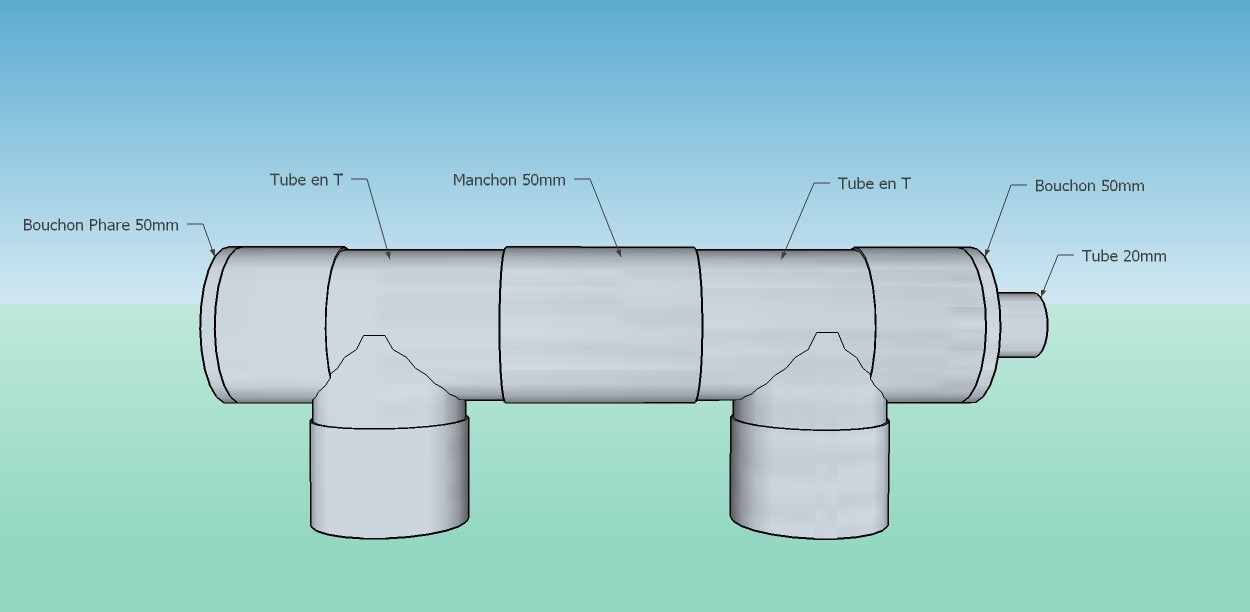
\includegraphics[scale=0.3]{ROVTubeSuperieur.jpg}
            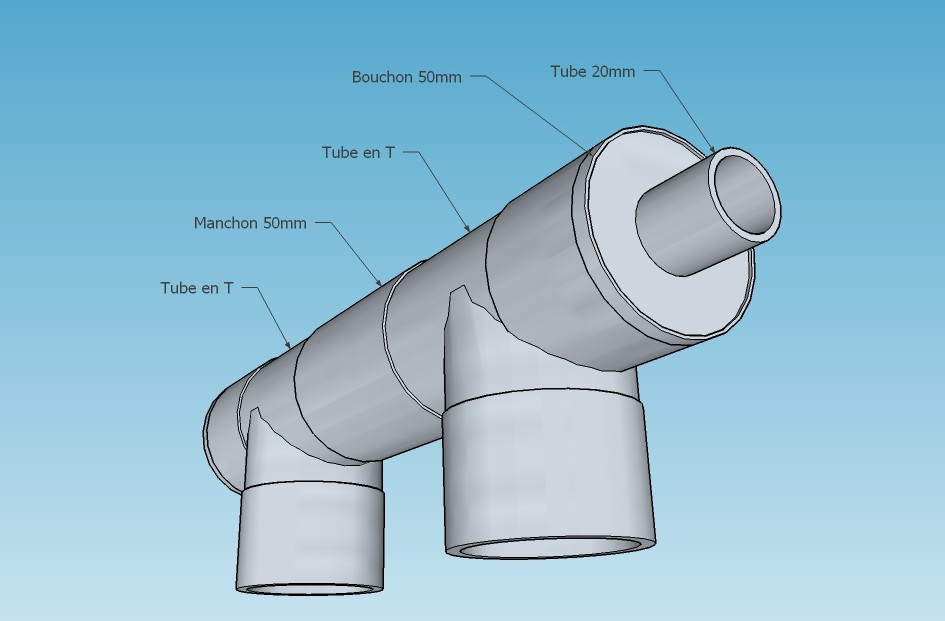
\includegraphics[scale=0.24]{ROVTubeSuperieurArriere.jpg}
            \caption{Tube supérieur.}
          \end{figure}
          
        \subsubsection{Pieds}
          \begin{enumerate}
            \item Procédez de la même manière que pour les tubes supérieurs : 2 tubes en T, 2 bouchons, 3 morceaux de tubes droit, le tout en diamètre 40mm. Collez les 4 pieds au tube principal. Inutile de le percer cette fois, vous devrez cependant adapter les tubes en contact avec la coque en fonction de la courbure de celle-ci.
            
            \item Vérifiez que la coque est droite en la posant sur une surface plate.
        \end{enumerate}
        
        \begin{figure}[H]
            \centering
            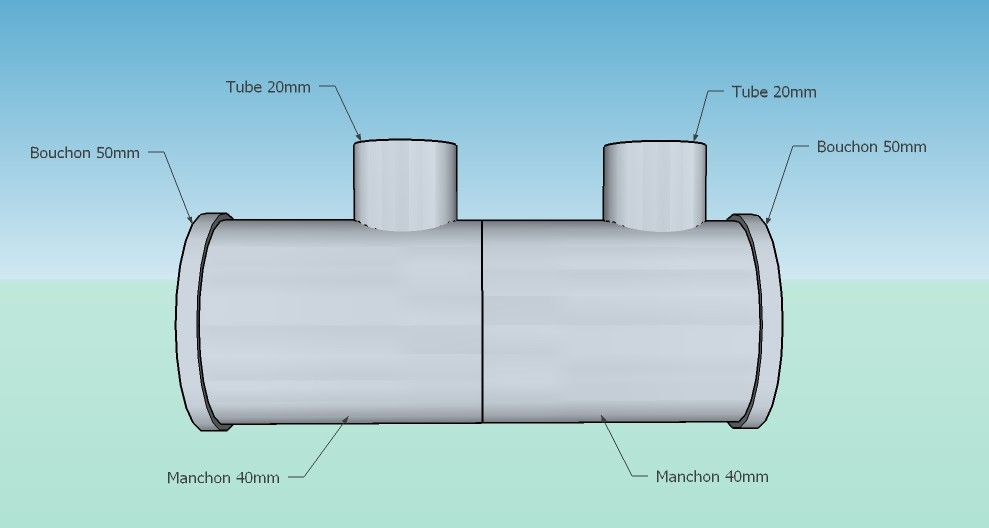
\includegraphics[scale=0.245]{ROVPiedCote.jpg}
            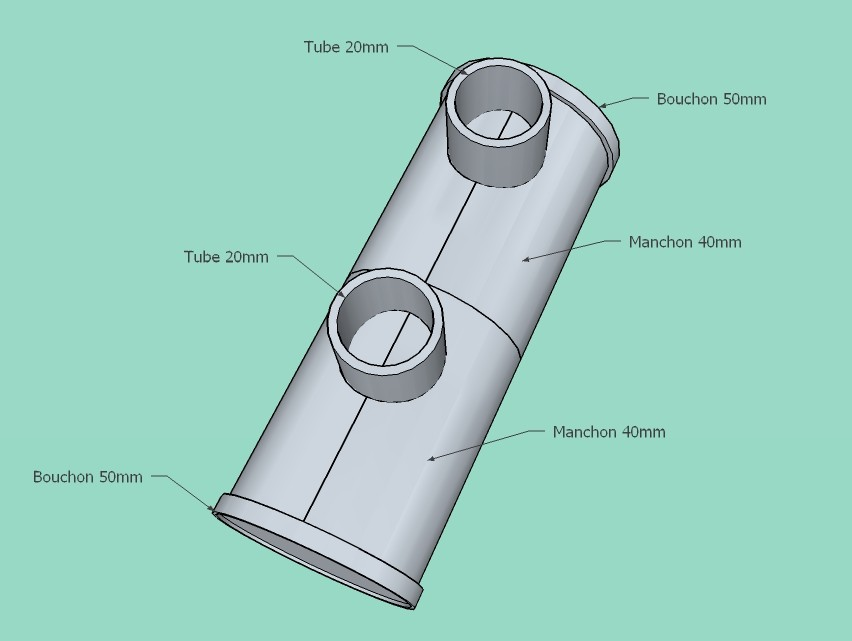
\includegraphics[scale=0.2]{ROVPiedHaut.jpg}
            \caption{Pied.}
          \end{figure}
        
        \subsubsection{Phares et entrée/sortie de la connectique}
          \begin{enumerate}
            \item Déterminez l'avant du ROV.
            \item Découpez un disque dans le bouchon avant d'un des tubes supérieurs, d'un rayon de 2cm environ (le même rayon que celui des ampoules LED en réalité).
            \item Découpez un disque en plexyglass de sorte qu'il puisse se loger sur le bouchon troué.
            \item Collez le disque de plexyglass sur le bouchon avec de la glue. Faites sécher en posant un objet lourd sur le disque de plexyglass afin de les serrer convenablement.
            \item Faites de même avec l'autre bouchon supérieur avant.
          \end{enumerate}
          
          \begin{figure}[H]
            \centering
            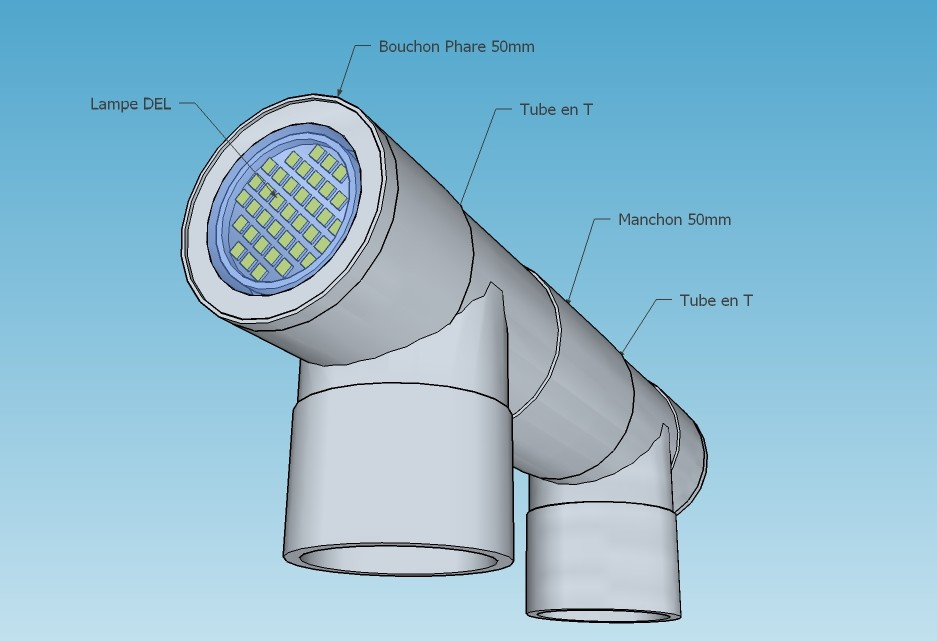
\includegraphics[scale=0.24]{ROVTubeSuperieurFace.jpg}
            \caption{Tube supérieur avec phare.}
          \end{figure}
          
          
        \subsubsection{Support caméra (optionnel)}
          \begin{enumerate}
            \item Découpez un tube PVC de diamètre 40mm de longueur 40mm puis coupez-le dans la longueur pour obtenir un U.
            
            \item Collez ce U sur la partie supérieure avant du tube principal, de façon à former un dôme. Vous pouvez visser votre support à caméra dans cette pièce sans compromètre l'étanchéité du ROV.
          \end{enumerate}
          
          \begin{remarque*}
            Le support caméra n'est pas présent sur le modèle 3D.
          \end{remarque*}

          
        \subsection{Moteurs et câble réseau}
          \begin{enumerate}
            \item Découpez deux morceaux de tube PVC de diamètre 20mm et de longueur 40mm.
            
            \item Percez les bouchons supérieurs arrières en leur centre pour faire passer ces tubes de 20mm.
            
            \item Faites passer une extrémité du rouleau de câble RJ45 à travers un tube de 20mm et glissez ce dernier dans le trou effectué dans un des deux bouchons. Collez le tube sur le bouchon en le laissant dépasser de 25mm à l'extérieur. Le câble doit dépasser sur une longueur d'environ 10cm.
            
            \item Remplissez le tube de colle époxy. Veillez à ce que le câble soit bien au milieu de la colle époxy lors du séchage, et non contre une paroi du tube.
            
            \item Collez de la même manière l'autre tube de 20mm au bouchon restant.
            
            \item Attachez les moteurs avec des colliers de serrage et de la ficelle aux endroit indiqués sur les photos. Vous pouvez aussi choisir de fabriquer des supports plus solides en PVC collés à la coque.
            
            \item Faites passer les fils des moteurs à travers le tube 20mm du dernier bouchon supérieur arrière et faites-les sortir par le tube principal de la coque (140mm) au travers de la jonction avec le tube supérieur (voir figure).
            
            \item Après avoir suffisamment tiré les fils pour laisser le moins de jeu possible (pas trop non plus!), remplissez de colle époxy le tube 20mm pour figer les fils moteurs. Attention : en collant les câbles, la torsion de ceux-ci lors du vissage du bouchon peut déterorier la colle époxy à long terme. Veillez à prendre en compte cette torsion lors du collage : il faut qu'aucune torsion ne soit appliquée sur les fils lorsque le bouchon est vissé.
            
          \end{enumerate}
          
          
        \begin{figure}[H]
          \centering
          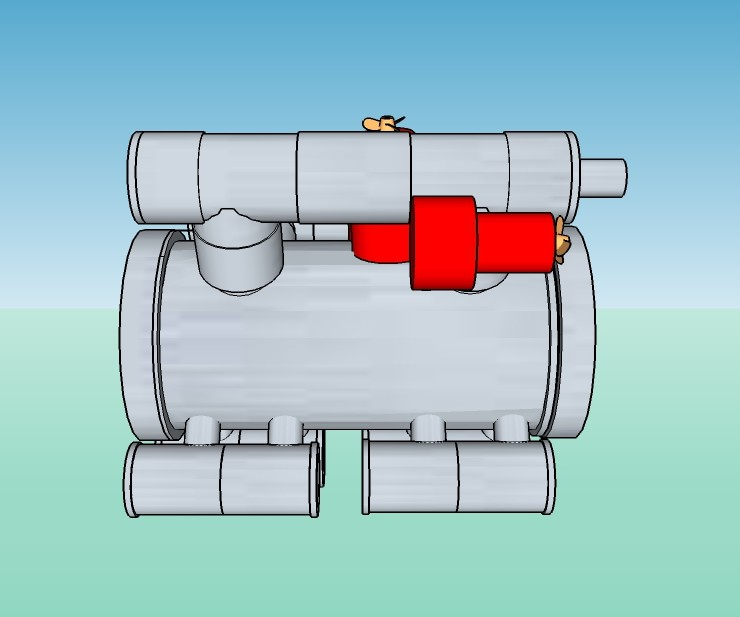
\includegraphics[scale=0.27]{ROVGauche.jpg}
          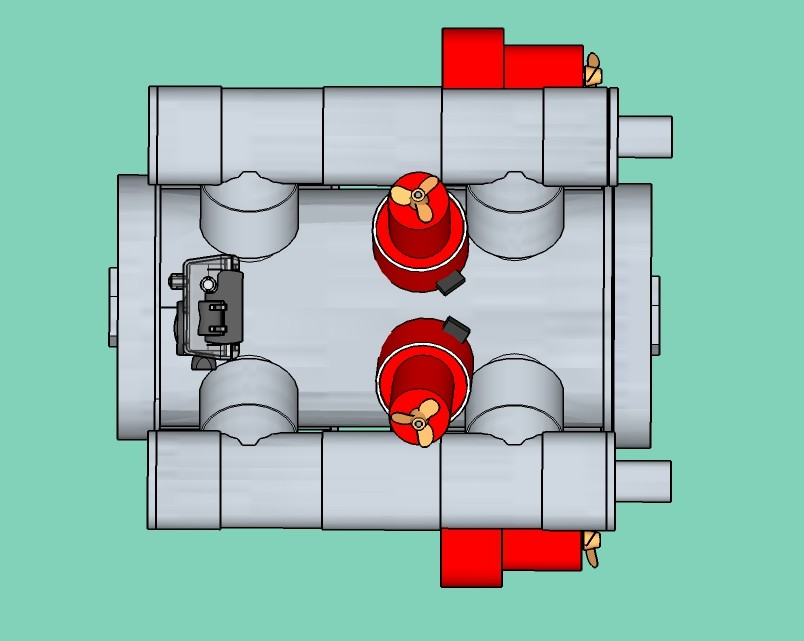
\includegraphics[scale=0.26]{ROVHaut.jpg}
          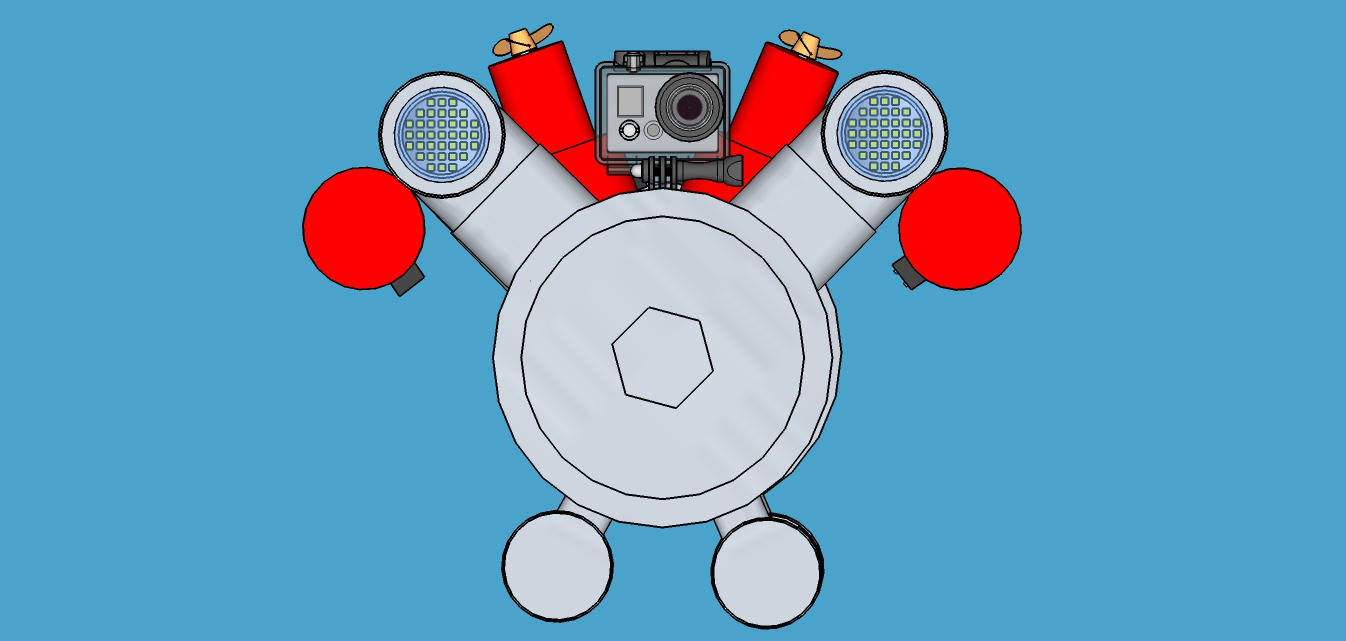
\includegraphics[scale=0.24]{ROVFace.jpg}
          \caption{Châssis interne.}
          \label{figChassis}
        \end{figure}

      \subsection{Télécommande}
        Le diamètre utilisé pour la télécommande est de 40mm. Cependant, j'ai rencontré des difficultés à rentrer les composants à l'intérieur donc je conseillerais plutôt un diamètre de 50mm.\\
        La longueur de la télécommande est de 15cm.
        \begin{enumerate}
          \item Assemblez deux manchons de PVC et terminez-le avec deux bouchons pour former un tube étanche: la télécommande.
          
          \item Découpez deux tubes de diamètre 40mm et de longueur 30mm.
          
          \item Percez la télécommande pour faire passer ces tubes en deux endroits distants de 6cm à 9cm (selon vos préférences).
          
          \item Collez les tubes à la télécommande de façon à ne rien laisser dépasser à l'intérieur. Au pire, vous réduirez la longueur des tubes par la suite.
          \item Découpez deux extrémités de doigt de gant de cuisine, retournez-les et placez sur les tubes perpendiculaires à la manette.
          
          \item Fixez les deux joysticks sur une baguette de 5mm x 5mm de longueur 13cm, en les séparant du même écart que celui choisi pour les tubes perpendiculaires à la manette. \\
          J'ai choisi d'orienter les broches vers le centre de la télécommande pour rassembler les fils.
          
          \item Connectez les fils aux joysticks et soudez-les aux broches d'un adaptateur femelle/femelle RJ45.% \footnote{voir la partie Câblage}
          
          \item Glissez le tout dans la télécommande et immobilisez-le si besoin. Testez l'accès aux joysticks au travers des tubes perpendiculaires. Pour ma télécommande, j'ai enlevé les coques arrondies des joysticks.
          
          \item Dans un des bouchons de la télécommande, procédez comme pour les bouchons supérieurs arrières de la coque, en y faisant traverser un tube de 20mm de diamètre et 30mm de long.
          
          \item Comme pour le premier bouchon supérieur arrière, faites passer une extrémité du rouleau de câble RJ45 à travers le tube de 20mm et glissez ce dernier dans le trou effectué du bouchon. Collez le tube sur le bouchon en le laissant dépasser de 25mm à l'extérieur. 
          
          \item Branchez le câble à l'adaptateur RJ45 de la télécommande.
          
          \item Notez la longueur de câble nécéssaire pour faire rentrer correctement les joysticks, les fils et l'adaptateur à l'intérieur de la télécommande. Puis remplissez le tube 20mm avec de la colle époxy pour figer le câble RJ45.
          
          \item Votre télécommande est prête!
        \end{enumerate}

      
      \subsection{Châssis interne}
        Longueur 127mm, Largeur : 116mm, Hauteur : 90mm.
        \begin{enumerate}
          \item Construisez le chassis selon le plan avec des baguettes 8mm x 8mm (Figure \ref{figChassis}).

          \item Calez la batterie avec du carton si besoin.
          
          \item Fixez les composants électroniques avec des vis 3mm et colliers de serrage (Figure \ref{figChassisComposants})..
          
          \item Ajoutez une rangée de 8 dominos sur la face arrière du chassis.
        \end{enumerate}
        
        \begin{figure}[H]
          \centering
          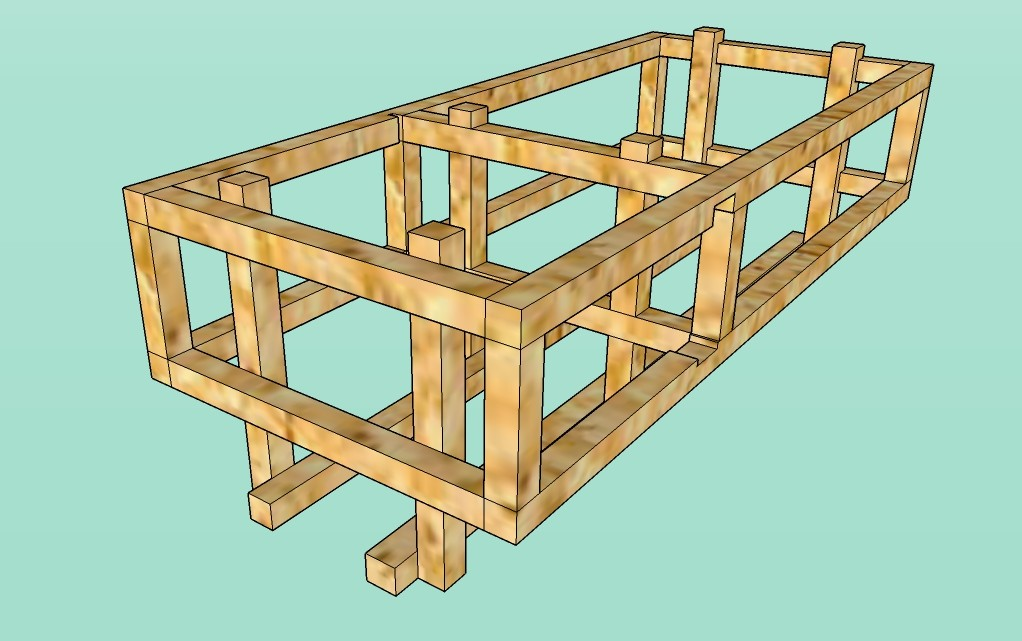
\includegraphics[scale=0.24]{ROVChassisGlobal.jpg}
          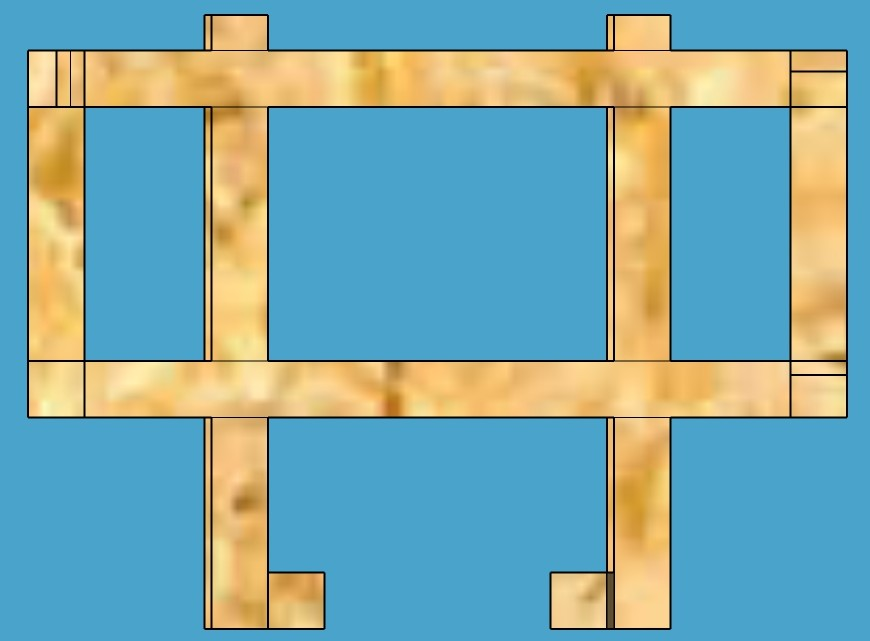
\includegraphics[scale=0.24]{ROVChassisFace.jpg}
          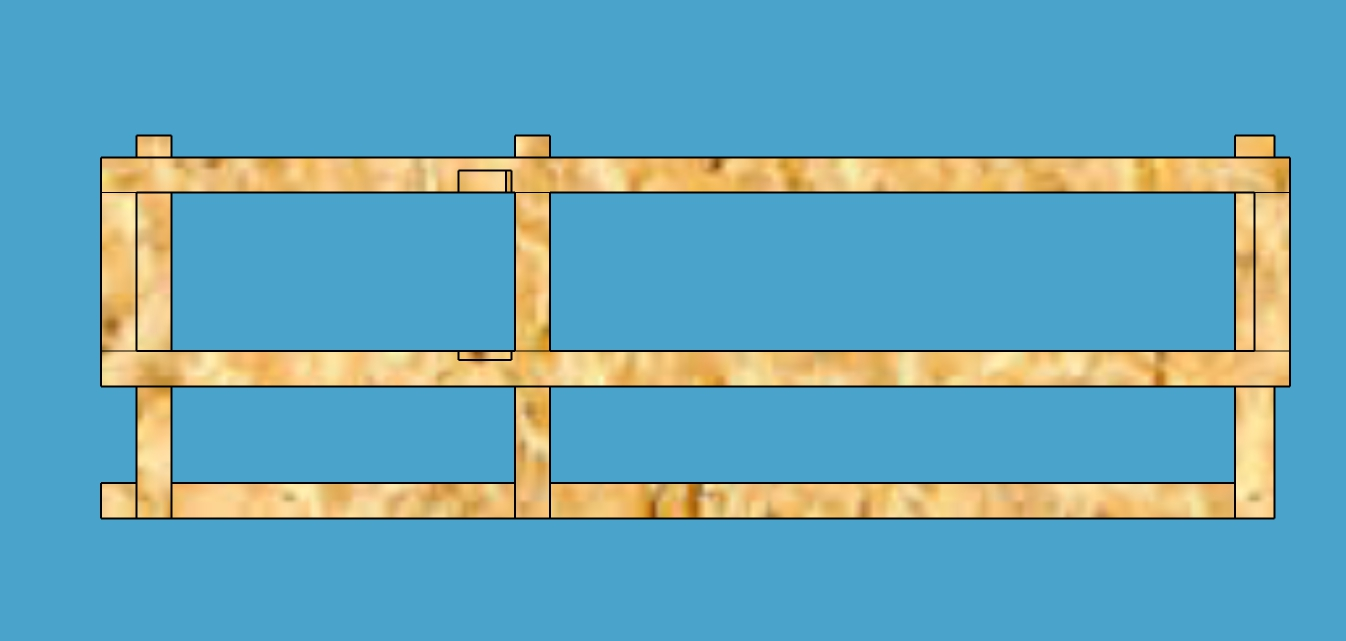
\includegraphics[scale=0.24]{ROVChassisGauche.jpg}
          \caption{Châssis interne.}
          \label{figChassis}
        \end{figure}
        \begin{figure}[H]
          \centering
          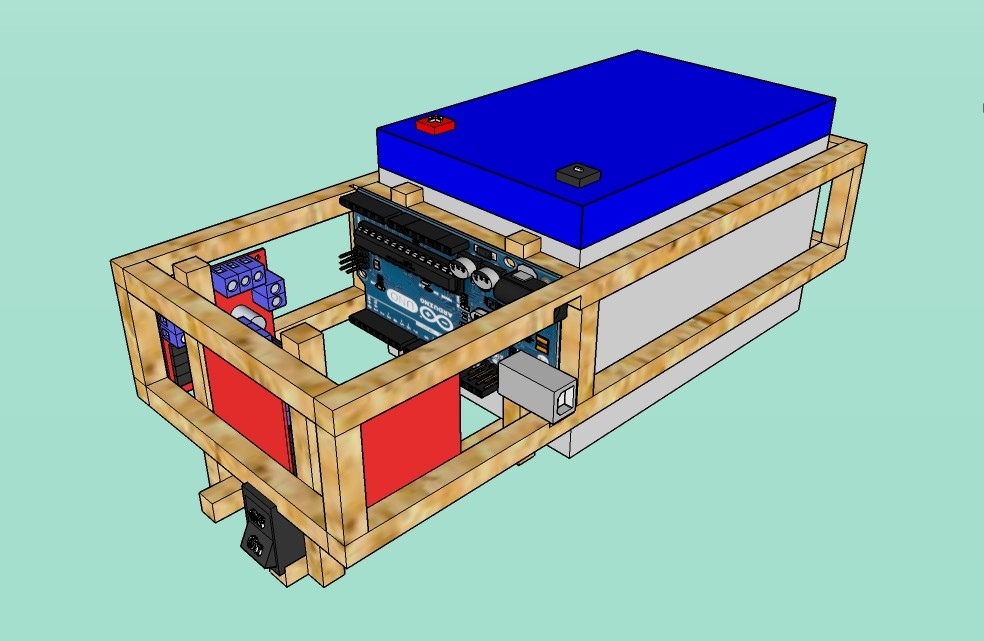
\includegraphics[scale=0.25]{ROVInterieurVueGlobale.jpg}
          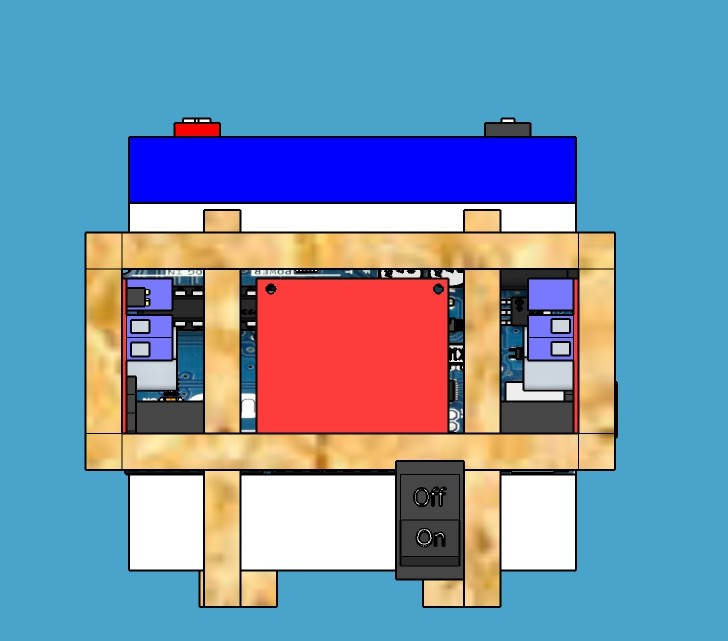
\includegraphics[scale=0.25]{ROVInterieurFace.jpg}
          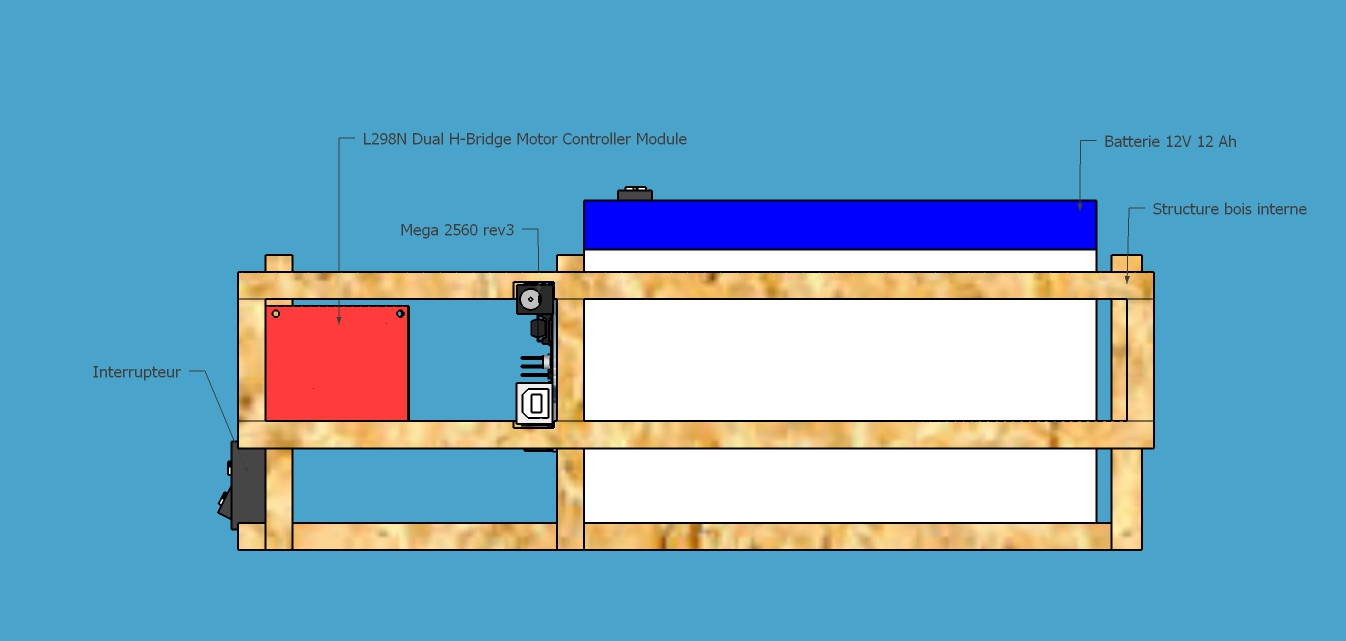
\includegraphics[scale=0.22]{ROVInterieurGauche.jpg}
          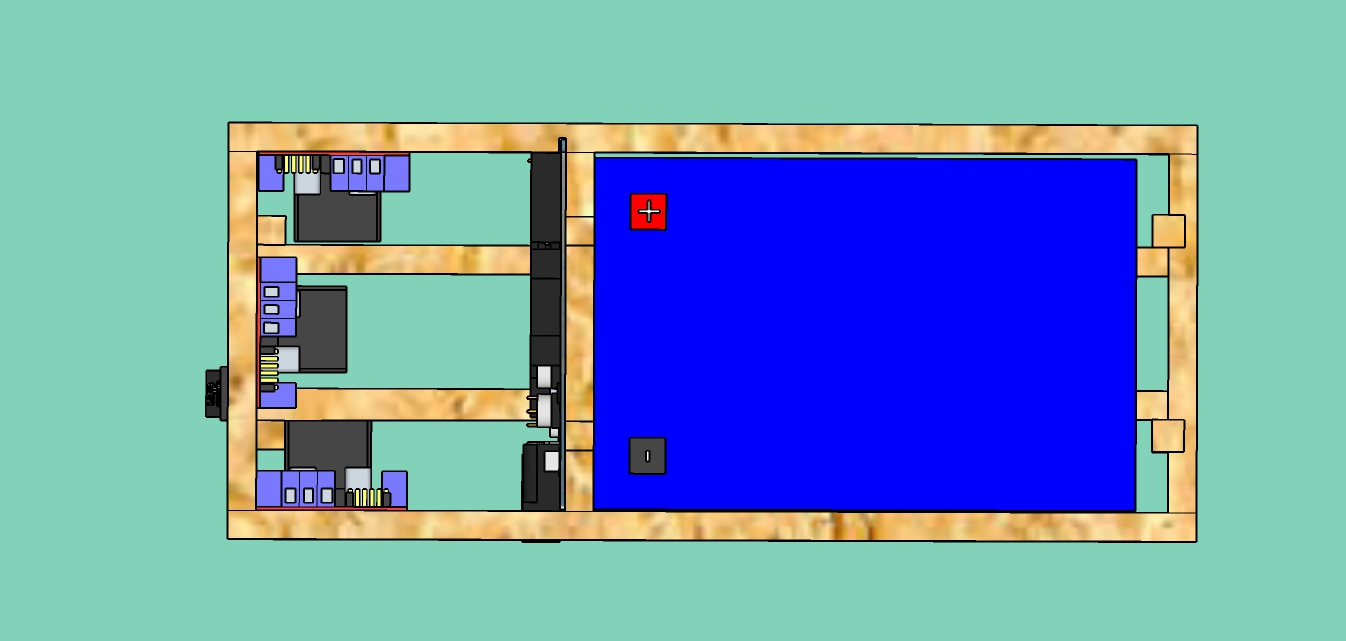
\includegraphics[scale=0.22]{ROVInterieurHaut.jpg}
          
          \caption{Châssis interne avec les composants.}
          \label{figChassisComposants}
        \end{figure}

      
      \subsection{Câblage}
        
        Voir le schéma global : Figure \ref{figConnexions}.
          \begin{remarque*}
            L'ensemble de mes fils étant scotchés entre eux (et par manque de rigueur au niveau de leur étiquetage), il m'a été difficile d'identifier certaines connexions. Cela ne concerne qu'une éventuelle inversion des pôles positifs et négatifs des moteurs. Il se peut donc que certaines connexions $\pm$ concernant les moteurs soient inversées. Cela a pour conséquence une rotation inverse de ces derniers. \\
            Dans tous les cas, je conseille de prendre ce schéma à titre d'exemple et de vérifier votre branchement en testant une à une chaque entrée/sortie de la carte de pilotage (en affichant les valeurs sur le port série par exemple).\\
            \textbf{Étiquetez les fils, cela vous épargnera de longues minutes à retrouver les bons branchement...}
          \end{remarque*}

          \begin{figure}[H]
            \centering
            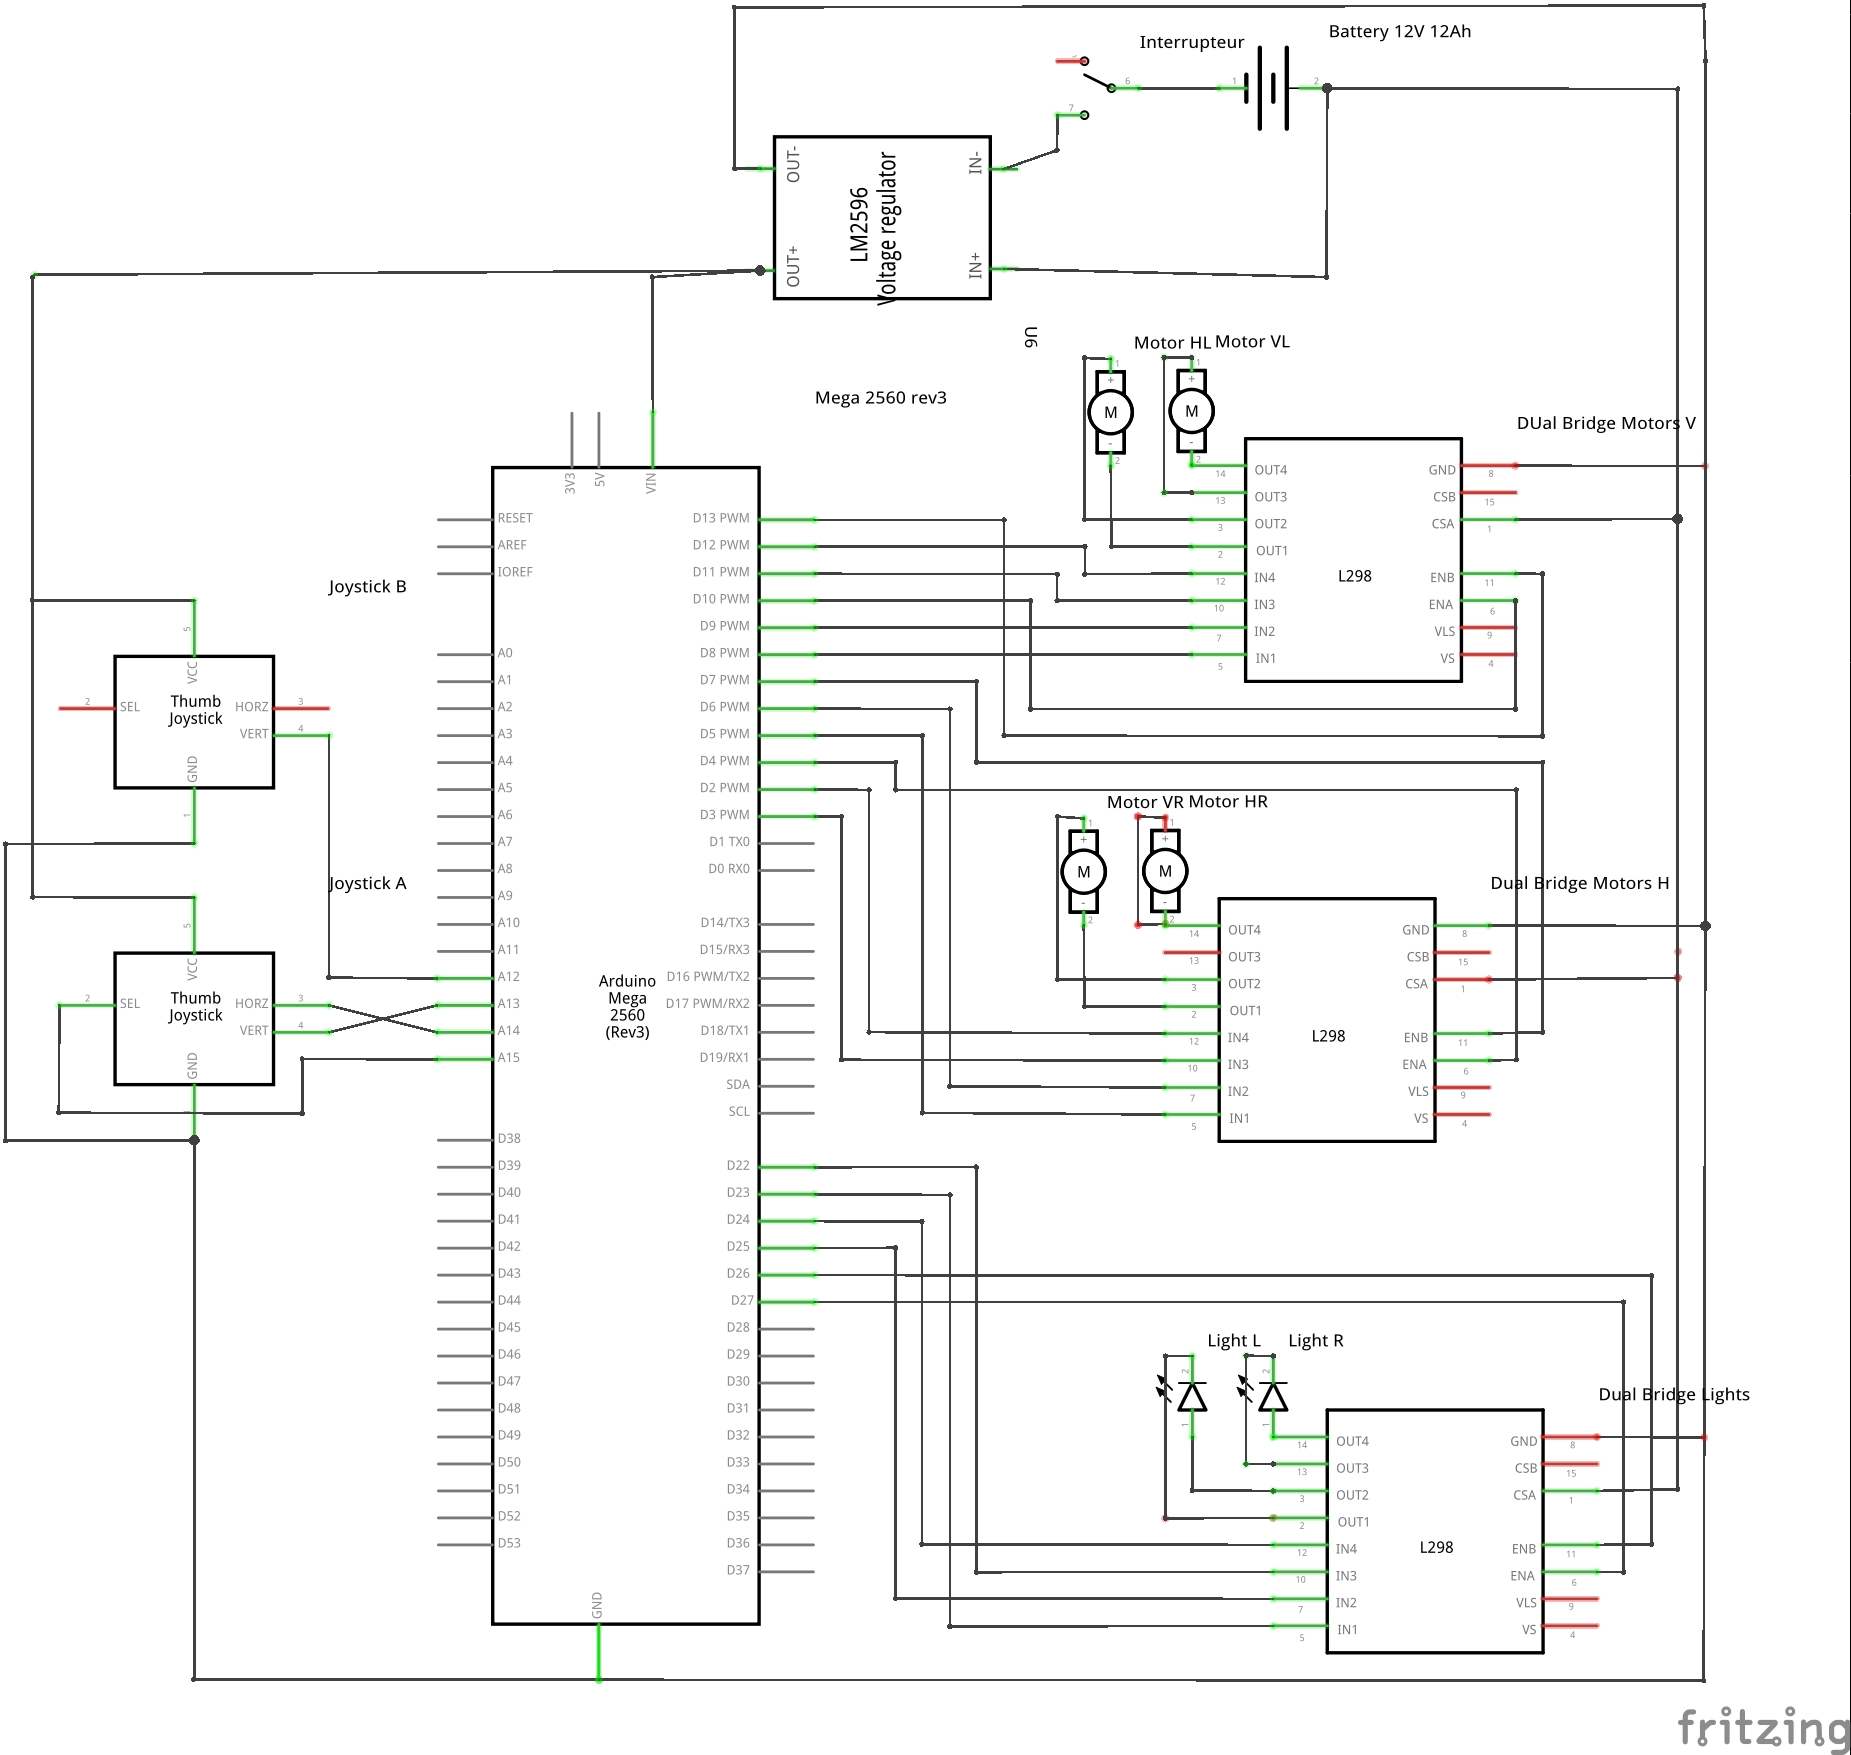
\includegraphics[scale=0.9]{schemaROV.jpg}
            \caption{Connexion entre les composants du ROV}
            \label{figConnexions}
          \end{figure}

      
        \subsubsection{Rallonge RJ45}
          La rallonge n'est rien d'autre qu'un câble réseau qui relie l'extrémité du rouleau RJ45 fixée au bouchon supérieur arrière à la carte de pilotage. 
          
          \begin{enumerate}
            \item Si vous possédez un câble RJ45 qui possède la bonne longueur, vous pouvez passez à l'étape suivante. Sinon, raccoursissez-en un à l'aide de pinces, fer à souder et gaines thermo-rétractables. Veillez à respecter les couleurs en soudant.
            \item Branchez chaque fiche RJ45 à un adaptateur.
            \item Branchez une extrémité du raccord à la fiche RJ45 correspondant à la télécommande.
          \end{enumerate}
          
        \subsubsection{Interfaces RJ45/Carte de pilotage et RJ45/Télécommande}
          Il s'agit de raccorder un câble RJ45 à un composant possédant des broches (femelles ou mâles). \\
          Ces interfaces ne sont pas nécessaires, elles ajoutent de la modularité au ROV. Vous pourrez simplement débrancher les fiches RJ45 pour une intervention sur le ROV au lieu de dessouder les fils ou débrancher les fils des composants et risquer d'oublier les correspondances.\\
          Vous pouvez choisir de ne pas en réaliser, il faudra simplement souder les fils à broches directement aux câbles du rouleau RJ45.
          
          \begin{enumerate}
            \item Découpez une fiche RJ45 en laissant suffisamment de longueur de fil (5cm -- 7cm maximum).
            
            \item En soudant, terminez chacun des fils du câble RJ45 par un fil muni d'une broche mâle. Ce dernier sera connecté aux broches femelles de la carte de pilotage. Vous obtenez votre interface RJ45/Carte de pilotage
            
            \item Procédez de la même manière pour construire l'interface RJ45/Télécommande en terminant avec des fils munis de broches femelles qui iront se connecter aux broches mâles des joysticks.
            
            \item Branchez les interfaces aux adaptateurs RJ45 aux extrémités du rouleau. 
            
          \end{enumerate}
        \subsubsection{Connexions}
          
      
      \section{Code arduino}
        Le code est disponible sur GitHub \url{XXXXX}. Bien que le code soit assez simple à comprendre, voici quelques explications concernant la liaison entre les joysticks et les moteurs :
        \begin{itemize}
          \item Fonctions \emph{double HL} et \emph{double HR}:
            \begin{itemize}
%               \item Rôle : reçoit les signaux des joysticks correspondants (joystick A pour le mouvement dans le plan horizontal, joystick B pour le mouvement vertical) et retourne un nombre entre -1 et 1 indiquant 
              \item Entrées \emph{(int X, int Y)} : valeurs comprises entre 0 et 1024 correspondant aux signaux X Y de sortie du joystick (A : pour le mouvement dans le plan horizontal, B : pour le mouvement vertical).
              \item Sortie  \emph{double res} : valeur comprise entre -1 et 1 indiquant la direction (positif : vers l'avant/haut, négatif : vers l'arrière/bas) ainsi que la vitesse (0 : aucune, 1 : maximale) du mouvement.
            \end{itemize}
            \item Partie \emph{// MOTORS //} dans la fonction principale \emph{void loop()}:\\ \emph{valHL} et \emph{valHR} récupèrent le nombre fourni par les fonctions \emph{HL} et \emph{HR}, compris entre -1 et 1. En fonction du signe de ces valeurs, le ROV avance ou recule, la vitesse étant contrôlée par la valeur absolue de ce nombre. Il en va de même pour les moteurs verticaux.
        \end{itemize}

    \section{Stabilisation}
      
      Si vous immergez le ROV à ce stade, vous observerez un sérieux déséquilibre de masse sur l'axe longitudinal (avant/arrière). En effet, l'arrière est  beaucoup trop lourd par rapport à l'avant à cause de la batterie et des moteurs. Il faut donc ajouter du poids à l'avant, tout en atteignant une flottaison nulle, pour que le ROV soit entre deux eaux. Cette partie est assez délicate et nécessite de la patience.
      \begin{enumerate}
        \item Remplissez d'eau une baignoire ou un bac assez grand pour accueillir le ROV.
        \item Glissez le châssis (avec batterie et composants) dans le tube principal et vissez bien tous les bouchons de visite. Les pieds doivent être aussi remplis d'air et hermétiquement fermés. Placez aussi la caméra (sa masse et son volume vont jouer dans la stablisation).
        \item Scotchez le plomb de plongée le plus à l'avant possible, entre les deux pieds.
        \item Immergez le ROV. 
        \begin{itemize}
          \item S'il flotte, ajoutez du plomb à l'avant.
          \item S'il coule mais que seuls les 2 pieds arrières touchent le sol, ajoutez du plomb à l'avant jusqu'à ce que les 4 pieds touchent le fond (vous pouvez ajouter du sable dans les pieds avant).
          \item Si le ROV coule et que les 4 pieds touchent le fond, il faudra ajouter un flotteur à l'arrière. C'est le tube horizontal situé sur le bouchon de visite arrière sur mon modèle. Attention : le volume de celui-ci doit être évalué avant de le fabriquer.
        \end{itemize}
        \item L'objectif est d'avoir un ROV qui, une fois immergé dans l'eau :
        \begin{itemize}
          \item reste dans le plan horizontal : pas de déséquilibre de masse dans l'axe longitudinal ni transversal
          \item ait une flottaison nulle ou très légèrement positive : le ROV doit rester au même endroit dans l'espace ou remonter très doucement vers la surface. Ainsi, si une panne survient au fond de l'eau, le ROV aura toujours tendance à remonter.
        \end{itemize}
      \end{enumerate}

      

    
    \section{Idées d'amélioration}
      \begin{enumerate}
        \item Augmenter la longueur du ROV pour permettre d'ajuster l'emplacement de la batterie pour régler le problème de centralisation de la masse.
        \item Ajouter un caisson pour webcam et un retour vidéo pour avoir un visuel en temps réel.
        \item Ajouter des pinces.
      \end{enumerate}


%         \begin{lstlisting}[style=Arduino]
% #include <VirtualWire.h>
% 
% double HL(int X, int Y)
% {
%   double res = 0;
%   int x = max(X,-511);
%   x = min(x,511);
%   int y = max(Y,-511);
%   y = min(y,511);
%   if (x+y>0)
%     res = min(x+y,512);
%   else
%     res = max(x+y,-512);
%   return res/512;
% }
% 
% double HR(int X, int Y)
% {
%   double res = 0;
%   int x = max(X,-511);
%   x = min(x,511);
%   int y = max(Y,-511);
%   y = min(y,511);
%   if (y-x>0)
%     res = min(y-x,512);
%   else
%     res = max(y-x,-512);
%   return res/512;
% }
% \end{lstlisting}
%   
%    \begin{lstlisting}[style=Arduino]
%     zadoakzd
%    \end{lstlisting}

    
%   
%   \section{Drone subaquatique avec caméra}
%     Liens:
%     \begin{itemize}
%       \item \href{http://www.instructables.com/id/Underwater-ROV/?ALLSTEPS}{Instructable}
%       \item \href{http://www.homebuiltrovs.com}{Homebuiltrovs}
%       \item \href{http://www.interspec.org/}{Interspec}
%       \item \href{http://www.rc-submarines.net/}{rc-submarines}
%       \item \href{http://www.mcmaster.com}{matériaux}
%       \item \href{http://www.diyrov.net/}{diyrov}
%       \item \href{http://stephane.lavirotte.com/perso/rov/esc_brushless_raspberry.html}{lien}: TUTO lier moteurs, esc et RPI
%       \item \href{http://explobotique.org/site/}{explobotique}
%       \item \href{http://uzzors2k.4hv.org/?page=rovnokken}{ROVNokken}
%     \end{itemize}
%     
%     \subsection{Pièces}
%     
%       \subsubsection{Propulsion}
% %         {\bf Solution 1}\\
% %         Source \url{http://www.homebuiltrovs.com/rovforum/viewtopic.php?f=3&t=1190} : 
% %         \begin{itemize}
% %           \item \href{http://hobbyking.com/hobbyking/store/__16229__NTM_Prop_Drive_Series_28_30A_750kv_140w.html}{DC motor} brushless :\\ 
% %           
% %             \begin{tabular}{ll}
% %               Model & NTM Prop Drive Series 28-30A 750kv\\
% %               Kv & 750rpm/v\\
% %               Max current & 20A\\
% %               Max Power &  120W @ 12v (3S) / 140W @ 15v (4S)\\
% %               Shaft & 3mm \\
% %               Weight & 67.1g\\
% %               ESC & 25A\\
% %               Cell count & 3s~4s Lipoly\\
% %               Bolt holes & 16mm \& 19mm\\
% %               Bolt thread&  M3\\
% %               Connection & 3.5mm Bullet-connector\\
% % %               Suggested Prop & Prop test data coming soon!
% % %               Prix: $4\times13.49= 53.96$ €
% %               Price & {\color{red} 13.49 €}
% %             \end{tabular}\\
% %           
% %           \item \href{http://hobbyking.com/hobbyking/store/__15205__Hobby_King_30A_ESC_3A_UBEC.html}{ESC}:\\
% %           \begin{tabular}{ll}
% %             Constant Current&  30A\\
% %             Burst Current & 40A\\
% %             Battery & 2-4S Lipoly / 5-12s NiXX\\
% %             BEC & 5v / 3A\\
% %             Motor Type & Sensorless Brushless\\
% %             Size & 54 x 26 11mm\\
% %             Weight & 32g \\
% %             Price & {\color{red} 8.99 €}
% %           \end{tabular}\\
% %           Programming Functions:\\
% %           \begin{tabular}{ll}
% %             Battery Type & Lipo /NiXX\\
% %             Brake & On / Off \\
% %             Voltage Protection & Low / Mid / High\\
% %             Protection mode & Reduce power / Cut off power \\
% %             Timing & Auto / High / Low\\
% %             Startup & Fast / Normal / Soft\\
% %             PWM Frequency & 8k / 16k \\
% %             Helicopter mode & Off / 5sec / 15sec (Start up delay)\\
% %           \end{tabular}
% % 
% %           
% %           \item \href{http://hobbyking.com/hobbyking/store/__7356__Turnigy_4mm_AquaProp_43x26x9mm_.html}{Propeller} :\\
% % 
% %           \begin{tabular}{ll}
% %             Model & Turnigy 4mm AquaProp\\
% %             Size & 43x26x9mm \\
% %             Length &   43mm\\
% %             Pitch &  26\\
% %             Diameter & 9mm \\
% %             Shaft Size & 4mm\\
% %             Price & {\color{red} 1.31 €}
% %           \end{tabular}
% %           
% % 
% %           \item \href{http://hobbyking.com/hobbyking/store/__12716__5mm_Drive_dog.html}{Dog drive}. Price {\color{red} $1.58$} €.
% % 
% %           \item \href{http://hobbyking.com/hobbyking/store/__16719__NTM_Prop_Drive_28_Series_Accessory_Pack.html}{Fixations}. Price {\color{red} $1.70$} €
% % 
% %         \end{itemize}
% %         
% %         Sous-total : $4\times 27.07 =$ {\color{red}$108.28$ €}
% %         
% %         
% %         {\bf Solution 2}\\
%         
%         \begin{itemize}
%           \item 4 \href{http://www.aliexpress.com/item/1100GPH-High-Flow-Submersible-Marine-Boat-Electric-Bilge-Pump-12V-3A-FREE-SHIPPING-DHL-EMS-gib/32302138453.html}{Pompes}. \PAYE\\
%                     \begin{tabular}{ll}
%                       Voltage & 12V \\
%                       Current & 3 Amp \\
%                       Flow rate & 1100GPH \\
%                       Height & Approx. 10.5cm\\
%                       Diameter & Approx. 5.5cm\\
%                       Weight & $\sim$ 300g? \\
%                       Price & {\color{red}13.21 €}
%                     \end{tabular}
%           
%           \item 4 \href{http://hobbyking.com/hobbyking/store/__12716__5mm_Drive_dog.html}{Dog dive}. Price {\color{red} $1.58$} €.
%           
%           \item 2 Dual H-bridge (30g Taille: 43 * 43 * 27mm) \PAYE \RECU
%           
%         \end{itemize}
%         Sous total {\color{red}$59.14$ €} 
% 
%         
% 
%         
%         
%       \subsubsection{Lumière \PAYE}
%         Référénce: une petite torche sous marine fait 300-600 lumens. 
%         \begin{itemize}
%           \item 2 \href{http://www.miniinthebox.com/fr/mr11-4-5w-15x5730smd-310-320lm-2800-3000k-chaud-ampoule-led-a-lumiere-blanche-spot-12-24v_p960936.html?pos=ultimately_buy_6}{ampoules} à DEL (Mass=?, 35 x 35 x 35 mm) à 4.5 W: $2\times 310 = 620$ lumens. Prix $2\times 2 =$ {\color{red}$4$ €}.
%           \item 1 Dual H-bridge (30g Taille: 43 * 43 * 27mm) \PAYE \RECU
%         \end{itemize}
% 
%         
%         
%         
%         
%       \subsubsection{Structure}
%       
%         \href{http://www.sitakiki.fr/modnaval/tuby.htm}{Lien}
%         \href{http://explobotique.free.fr/vidi1/vidi1_detail3.htm}{vidi}
%         \href{http://explobotique.free.fr/ptipi/realisation_hublot.htm}{hublot}
%         \begin{itemize}
%           \item 1 \href{http://www.pointp.fr/gros-oeuvre-vrd-tp/tube-pvc-sotrabat-nf-me-gris-diametre-140mm-longueur-4m-eu-ep-A3890917p213S2R2m23}{tube} PVC 1000x140mm. Prix: {\color{red}7.98 €}
%           \item 2 tubes 
%         \end{itemize}
% 
%       
%       \subsubsection{Télécommande  \PAYE}
%         Télécommande reliée par fils, submersible, composée de 2 joysticks : 1 pour le plan horizontal, 1 pour l'axe vertical. Éventuellement un contrôle on/off global et un autre pour l'éclairage.\\
%         \begin{itemize}
%           \item 2 \href{http://www.ebay.co.uk/itm/Analogue-Joystick-Controller-5V-With-Click-Button-Arduino-PI-Compatible-/191608236635?}{Joysticks} Prix : {\color{red} 4.20 €} \PAYE
%           \item câble ethernet \RECU
%         \end{itemize}
% 
% 
%         BONUS: Activation de la prise de photo/vidéo par servos. 2 \href{http://www.miniinthebox.com/fr/mini-servo-9g-avec-accessoires-bleu-translucide_p638990.html?litb_from=sysmail}{servos} et leurs fixations. Prix $2\times 2.59=$ {\color{red}$5.18$ €} \PAYE.
%       
%       \subsubsection{Électronique  \PAYE}
%         \begin{itemize}
%           \item \href{http://www.amazon.fr/LM2596-Abaisseur-Régulateur-Tension-Ajustable/dp/B00GSY3UBS/ref=pd_cp_147_1?ie=UTF8&refRID=19H2WCT90TTWCF32P1HK}{Régulateur} tension (Mass=?, 48 x 23 x 14 mm). Prix : {\color{red} 1.80 €}.
%           \item \href{http://www.miniinthebox.com/fr/mega-2560-conseil-du-developpement-r3-conseil-atmega2560-16au-pour-arduino_p903300.html}{Arduino Mega 2560 R3}. \\
%           \begin{tabular}{ll}
%             
%           
%             Length & 101.98mm \\
%             Width & 53.63mm \\
%             Height & 15.29mm \\
%             Weight & 34.9g\\
%             Price: {\color{red}$9.99$ €}.
%           \end{tabular}
%           
%           
%           
%           \item 2 \href{http://www.ebay.fr/itm/2-modules-detection-pluie-eau-Water-Sensor-pour-Arduino-envoi-de-France-E137-/201370405351?pt=LH_DefaultDomain_71&hash=item2ee29c89e7}{Capteurs} niveau d'eau (4.7g, 20 x 40 mm). Prix {\color{red} 3,69 €} \PAYE.
%         \end{itemize}
%         Test du cable ethernet : 5m OK.
% 
%         
%       
%       \subsubsection{Batterie \PAYE}
%         12V, plus de 3 Ah
%         \begin{itemize}
%           \item \href{http://www.amazon.fr/gp/product/B001CNZP6S?psc=1&redirect=true&ref_=od_aui_detailpages00}{Chargeur} 3, 6, 12V,  3,4 KG. Prix: {\color{red} 16,25 €}.
%           \item \href{http://www.amazon.fr/Batterie-plomb-AGM-12V-12Ah-12Ah/dp/B008FZ0WEG}{Batterie} plomb étanche AGM, $151 \times 98 \times 95$ mm, 12V 12Ah. Prix: {\color{red} 18,90 €}.
%         \end{itemize}
%         %\underline{ATTENTION}: dégage de l'hydrogène: isoler du reste des composants électroniques!
%         
%     \subsection{Calcul volume total d'air requis}
%       Il s'agit d'avoir une idée de la taille globale du ROV. On le modélise par un cylindre en PVC fermé avec deux bouchons en PVC.
%       Masse des composants (g):\\

  \bibliographystyle{plain}
  \bibliography{sources}
      
\end{document}



